% -*- coding: UTF-8 -*-
\documentclass[twoside,nofonts,fancyhdr,openany,UTF8,fleqn]{ctexart} % 设置文章类型
\usepackage{CJK}
\usepackage{amsmath}
\usepackage{amssymb}
\usepackage{graphicx}				% 调用插图宏包
\usepackage[colorlinks,linkcolor=red]{hyperref}  % 添加链接的宏包
\pagestyle{empty}					% 无页眉页脚格式

% 设置字体
\setCJKmainfont[AutoFakeBold=true]{Adobe Song Std} 
\setCJKsansfont{Adobe Heiti Std}
\setCJKmonofont{Adobe FangSong Std}
\graphicspath{ {images/} }		% 指定图片路径

\title{CS24N Assignment1}    	% 标题
\author{Jerry.Shi}		% 作者

\begin{document}	% 正文开始

%\maketitle			% 制作封面

%\tableofcontents % 加入目录,包括页码

\section{Softmax}
\subsection{a}
证明softmax函数对于任意的向量\textbf{\emph{x}} 和任意常数\emph{c}存在以下关系,
\begin{equation}
softmax(\textbf{\emph{x}}) = softmax(\textbf{\emph{x}} + \emph{c})
\end{equation}
上式表示对向量的每个维度同时加上同一个常数softmax的结果不变,softmax公式如下,
\begin{equation}
softmax(\textbf{\emph{x}})_i = \frac{exp(\emph{x}_i)}{\sum_{j}exp(\emph{x}_j)}
\end{equation}
一般情况下为了保持数值稳定性会选择$\textbf{c}=-\textbf{max}(\textbf{\emph{x}}_i)$, 让每个维度都减去最大的那个元素,进行稳定性处理。

\textbf{Soultion}:
根据softmax的公式得到,
% 推导过程

\begin{align}
softmax(\textbf{\emph{x}+c})  & =  \frac{exp(\textbf{x}_i + \textbf{c})}{\sum_{j}exp(\emph{x}_j+\textbf{c})} \\
								  & =  \frac{exp(\textbf{x}_i)exp(\textbf{c})}{\sum_{j}exp(\emph{x}_j)exp(\textbf{c})}	\\
								  & = \frac{exp(\textbf{x}_i)}{\sum_{j}(exp(\emph{x}_))}	\\
								  & = softmax(\textbf{\emph{x}}) 
\end{align} % 这里不要有空行否则会出错

\subsection{b}
给定一个\textbf{N}x\textbf{D}的矩阵,使用题目a中的特性求解矩阵中每一行的softmax结果,在文件q1softmax.py中给出实现和测试。


% 第二节
\section{Neural Network Basics}
% a
\subsection{a}
推导sigmod函数的梯度,并将其表示成其他函数的形式,sigmod函数如下,
\begin{equation}
 \sigma(\textbf{x}) = \frac{1}{1+exp(-\textbf{x})} 
\end{equation}
\textbf{Soultion}:
\begin{align}
\sigma^\prime(\textbf{x})  & = \frac{exp(-\textbf{x})}{(1+exp(-\textbf{x}))^2} \\
		& = \frac{1}{1+exp(-\textbf{x})}\frac{exp(x)}{1+exp(-\textbf{x})} \\
	& = \frac{1}{1+exp(-\textbf{x})}(1- \frac{1}{1+exp(-\textbf{x})})	\\
	& = \sigma(\textbf{x})(1-\sigma(x))
\end{align}

% b
\subsection{b} 
推导激活函数为softmax,loss 为 cross entropy的情况下,输入向量$\theta$,求loss对输入$\theta$的梯度。预测结果$\hat{\textbf{\emph{y}}}=softmax(\theta)$,交叉熵cross entropy公式为,
\begin{equation}
CE(\textbf{\emph{y}}, \hat{\textbf{\emph{y}}}) = - \sum_{i}y_ilog(\hat{y}_i)
\end{equation}

其中向量\textbf{\emph{y}}为one-hot编码,$\hat{\textbf{\emph{y}}}$是对所有class的预测概率向量。

\textbf{Soultion}:
对$\theta$求导
首先根据softmax函数定义,
\begin{equation}
\widehat{y_i} = softmax(\theta_{i}) = \frac{exp(\theta_{i})}{\sum_{k=1}{exp(\theta_{k})}} = \frac{u_i}{v_i}=f_i
\end{equation}
把$f_i$当成是两个函数$u_i$和$v_i$复合结果,在当前情况下i可以理解为y中第i个元素的预测结果。下面推导$f_i$对$\theta_j$的求导。
\begin{equation}
\frac{\partial{f_i}}{\partial{\theta_j}} = \frac{u_{i}^{\prime}v_j-u_{i}v_{i}^{\prime}}{(v_i)^2}
\end{equation}

此时不能直接进行计算求导,因为不清楚i和j是否相等,因此需要分情况考虑。
当\textbf{i=j}时,此时由
\begin{equation}
u_{i}^{\prime}=\frac{\partial{u_i}}{\partial{\theta_j}}=exp(\theta_i) \\
v_{i}^{\prime}=\frac{\partial{v_i}}{\partial{\theta_j}}=exp(\theta_j)	\\
\end{equation}
将结果代入求导结果
\begin{align}
\frac{\partial{f_i}}{\partial{\theta_j}} 		\\
	& = \frac{u_{i}^{\prime}v_j-u_{i}v_{i}^{\prime}}{(v_i)^2} \\
	& = \frac{exp(\theta_i)\sum_{k=1}{exp(\theta_k)}-exp(\theta_i)exp(\theta_j)}{\sum_{k=1}{exp(\theta_k)}\sum_{k=1}{exp(\theta_k)}}	\\
& = \frac{exp(\theta_i)}{\sum_{k=1}{exp(\theta_k)}}\frac{\sum_{k=1}{exp(\theta_k)}-exp(\theta_j)}{\sum_{k=1}{exp(\theta_k)}} \\
& = f_i(1-f_j) \\
& = f_i(1-f_i)
\end{align}

当\textbf{i!=j}时,结果为
\begin{equation}
u_{i}^{\prime}=\frac{\partial{u_i}}{\partial{\theta_j}}=0 \\
v_{i}^{\prime}=\frac{\partial{v_i}}{\partial{\theta_j}}=exp(\theta_j)	\\
\end{equation}
将结果代入可得

\begin{align}
\frac{\partial{f_i}}{\partial{\theta_j}} = \frac{0-u_{i}v_{i}^{\prime}}{(v_i)^2}	\\
& = - \frac{exp(\theta_i)}{\sum_{k=1}{exp(\theta_k)}}\frac{exp(\theta_j)}{\sum_{k=1}{exp(\theta_k)}}	\\
& = -f_{i}f_j
\end{align}

结合以上求导结果求交叉熵对$\theta_i$的梯度
\begin{align}
\frac{\partial{CE(y_k,\widehat{y_k})}}{\partial{\theta_i}} \\
	& = -\frac{\partial{\sum_{k=1}{y_klog(\widehat{y_k})}}}{\partial{\theta_i}} \\
	& = -\sum_{k=1}y_{k}\frac{1}{f_k}\frac{\partial{f_k}}{\partial{\theta_i}} \\
	& = -y_i(1-f_i)-\sum_{k\neq{i}}y_{k}\frac{1}{f_k}(-f_{k}f_{i})	\\
	& = -y_i + y_{i}f_{i}+\sum_{k\neq{i}}y_{k}f_{i}	\\
	& = -y_i + \sum_{k=1}y_{k}f_{i}	\\
	& = \widehat{y_i} - y_i
\end{align}
在推导过程中主要考虑k和i相等、不相等两种情况。

% c
\subsection{c}
对三层网络如图,推导误差对输入梯度$\frac{\partial{J}}{\partial{x}}$,$J=CE(y,\widehat{y})$。
隐藏层采用sigmod作为激活函数,输出层采用softmax作为,y采用one-hot编码。可用公式如下,
$$h = sigmod(xW_1 + b_1) \\ \widehat{y} = softmax(hW_2 + b_2)$$
% image
\begin{figure}[!htb]
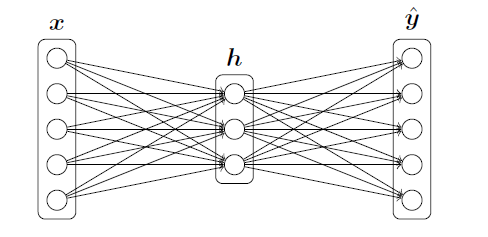
\includegraphics[scale=0.5]{assign_1}
\centering
\caption{}
\end{figure}

\textbf{Soultion}:
根据误差反向传播算法,误差对输入x的导数,等于从输出到输入反向情况下,所有节点的输出对输入导数的累乘。做如下定义,
$z_1 = W_1x + b_1 \\ \widehat{y}=W_2h + b_2 \\ h = sigmod(z_1)=\sigma(z_1)$
则误差对输入的导数为,
\begin{align}
\frac{\partial{CE}}{\partial{x}} = \frac{\partial{CE}}{\partial{\widehat{y}}}\frac{\partial{\widehat{y}}}{\partial{h}}\frac{\partial{h}}{\partial{z_1}}\frac{\partial{z_1}}{\partial{x}} \\ 
	& = (\widehat{y}-y)W_{2}^{T}\circ\sigma^{\prime}(z_1)W_{1}^{T}
\end{align}

\subsection{d}
如果输入是$D_x$维向量,隐藏层单元数为H,计算该网络所需要的参数数量。
\textbf{Solution}:
由于输入x到隐藏层是全连接,每个维度都与H个单元向量相连,且都有bias存在,因此有$(D_x + 1)\times H$个参数,同理,隐藏层与$D_x$个输出单元相连,再加上bias有$(H + 1)\times D_x$,因此该网络总共有参数,$(D_x +1)\times H + (H+1)\times D_y$
\subsection{e,f,g属于编程实现}

% 3
\section{word2vec}
% 3.a
\subsection{a}
基于word2vec中skipgram 模型,给定中心词word c的预测结果$v_c$,输出采用softmax,误差采用cross entropy,求误差对$v_c$的梯度。
\textbf{Solution}:
设$y$和$\widehat{y}$均是列向量。
\begin{align}
J = CE \\ 
& = -{y_i}log(\widehat{y_i}) \\
& = -log(\frac{exp(u_o^Tv_c)}{\sum_{w=1}^{T}exp(u_w^Tv_c)}) \\
& = -u_o^Tv_c + log({\sum_{w=1}^{|W|}exp(u_w^Tv_c)})
\end{align}

误差对输入的梯度:
\begin{align}
\frac{\partial{CE}}{\partial{v_c}}  \\
& = -u_o + \frac{1}{\sum_{w=1}^{T}exp(u_w^Tv_c)}\frac{\partial}{\partial{v_c}}{\sum_{i=1}^{T}exp(u_i^Tv_c)} \\
& = -u_o + \sum_{i=1}^{W}\frac{exp(u_i^Tv_c)}{\sum_{w=1}^{W}exp(u_w^Tv_c)}u_i \\
& = -u_o + \sum_{i=1}^{W}\widehat{y_i}u_i
\end{align}

% 3.b
\subsection{b}
根据上个题目的情况,对$u_w$求梯度(包括$u_o$).
\begin{align}
J = CE \\ 
& = -{y_i}log(\widehat{y_i}) \\
& = -log(\frac{exp(u_o^Tv_c)}{\sum_{w=1}^{T}exp(u_w^Tv_c)}) \\
& = -u_o^Tv_c + log({\sum_{w=1}^{|W|}exp(u_w^Tv_c)})
\end{align}

当$o=w$时,梯度结果为
\begin{align}
\frac{\partial{CE}}{\partial{u_w}} \\
	& = -v_c + \frac{1}{\sum_{w=1}^{W}exp(u_w^Tv_c)}\frac{\partial}{\partial{u_w}}\sum_{i=1}^{W}exp(u_i^Tv_c) \\
& = -v_c + \frac{exp(u_w^Tv_c)}{\sum_{w=1}^{W}exp(u_w^Tv_c)}v_c \\
& = (\widehat{y_w}-1)v_c
\end{align}
当$o\neq{w}$,
\begin{align}
\frac{\partial{CE}}{\partial{u_w}} \\
	& = \frac{1}{\sum_{w=1}^{W}exp(u_w^Tv_c)}\frac{\partial}{\partial{u_w}}\sum_{i=1}^{W}exp(u_i^Tv_c) \\
& = \frac{exp(u_w^Tv_c)}{\sum_{w=1}^{W}exp(u_w^Tv_c)}v_c \\
& = \widehat{y_w}v_c
\end{align}

所以,
\begin{align}
\frac{\partial{CE}}{\partial{u_w}} = \left \{ 
\begin{aligned}
(\widehat{y_w}-1)v_c , o=w\\
\widehat{y_w}v_c , otherwise
\end{aligned}
\right.
\end{align}


\end{document}
